% VLDB template version of 2020-08-03 enhances the ACM template, version 1.7.0:
% https://www.acm.org/publications/proceedings-template
% The ACM Latex guide provides further information about the ACM template
\usepackage[spanish]{babel}

\documentclass[sigconf, nonacm]{acmart}

%% The following content must be adapted for the final version
% paper-specific
\newcommand\vldbdoi{XX.XX/XXX.XX}
\newcommand\vldbpages{XXX-XXX}
% issue-specific
\newcommand\vldbvolume{14}
\newcommand\vldbissue{1}
\newcommand\vldbyear{2020}
% should be fine as it is
\newcommand\vldbauthors{\authors}
\newcommand\vldbtitle{\shorttitle} 
% leave empty if no availability url should be set
\newcommand\vldbavailabilityurl{http://vldb.org/pvldb/format_vol14.html}
% whether page numbers should be shown or not, use 'plain' for review versions, 'empty' for camera ready
\newcommand\vldbpagestyle{plain} 

\begin{document}
\title{ESTUDIO DEL MÉTODO MONTE CARLO EN SIMULACIONES PARA LA ESTIMACIÓN DEL VALOR DE PI}

%%
%% The "author" command and its associated commands are used to define the authors and their affiliations.
\author{Juan Pablo Crespo Vargas}
\affiliation{%
  \institution{Sensei Dojo Cobra Py}
  \streetaddress{https://github.com/CobraPython}
  \city{La Paz}
  \state{Bolivia}
}
\email{jp.crespo.vargas@gmail.com}


\author{Donald Fauntleroy Duck}
\affiliation{%
  \institution{Scientific Writing Academy}
  \city{Duckburg}
  \country{Calisota}
}
\email{donald@swa.edu}

%%
%% The abstract is a short summary of the work to be presented in the
%% article.
\renewcommand{\abstractname}{Resumen}
\begin{abstract}
En este artículo se presenta los resultados de tres metodologías diferentes en las que se aplicó una simulación Monte Carlo para estimar el valor de Pi: el método de comparación de áreas, el método propuesto por Buffon y la extensión de Laplace. Los tres casos se desarrollaron en un lenguaje de alto nivel, Python y la librería Numpy que le otorgan un performance optimizado. Se estudió con detalle el resultado no determinista de las simulaciones y se demostró que cumplen con los teoremas fundamentales de la probabilidad.
\end{abstract}

\maketitle


%%% do not modify the following VLDB block %%
%%% VLDB block start %%%
\ifdefempty{\vldbavailabilityurl}{}{
\vspace{.3cm}
\begingroup\small\noindent\raggedright\textbf{Palabras Clave}\\
Simulación, Monte Carlo, Pi, Buffon, Buffon-Laplace, Python, Numpy.
\endgroup
}
%%% VLDB block end %%%

\section{INTRODUCCIÓN}

El método de Monte Carlo tiene un génesis moderno en el trabajo pionero de Stan Ulam y John Von Neumann. Luego de la segunda Guerra Mundial aplicaron distintos métodos de Monte Carlo en simulaciones para el desarrollo de armas termonucleares. Desde entonces y por más de 50 años que se aplicaron estos desarrollos en la investigación y perfeccionamiento de distintos métodos que modelan el transporte de neutrones y radiación gamma con bastante éxito experimental.\cite{Andreas}
Hoy resulta una alegre ironía que ningún producto que haya aplicado la metodología Monte Carlo en su desarrollo, se haya empleado en conflicto alguno. Más aún los científicos han explotado el uso de simulaciones Monte Carlo para obtener un beneficio público positivo aplicándola en salud. Por ejemplo, los planeamientos de dosis en radioterapia dependen actualmente en algún grado de cálculos obtenidos mediante simulaciones Monte Carlo. 
El método de Monte Carlo es un método de resolución numérica donde se modelan las relaciones e interacciones de distintos objetos y su entorno, mediante la generación aleatoria de estas interacciones. Mientras mayor sea la repetición de pruebas se obtiene un resultado que va convergiendo a un valor con mayor precisión. Es por el recurso de la aleatoriedad que obtiene el nombre Monte Carlo, pues se inspira en la región del Principado de Mónaco donde se encuentran el casino Monte Carlo. 
Un método Monte Carlo se puede definir de la siguiente forma: <<Los métodos Monte Carlo son aquéllos en los que las propiedades de las distribuciones de las variables aleatorias son investigadas mediante la simulación de números aleatorios. Estos métodos, dejando a un lado el origen de los datos, son similares a los métodos estadísticos habituales en los cuales las muestras aleatorias se utilizan para realizar inferencias acerca de las poblaciones origen. Generalmente, en su aplicación estadística se utiliza un modelo para simular un fenómeno que contiene algún componente aleatorio. En los métodos Monte Carlo, por otro lado, el objeto de la investigación es un modelo en sí mismo, y se utilizan sucesos 
aleatorios o pseudoaleatorios para estudiarlo.>> \cite{Gentle}

El método cobra una especial relevancia las últimas décadas debido a que se produjeron sustanciales y significativos avances respecto a la potencia de los procesadores y las distintas arquitecturas informáticas. Es ampliamente usado en problemas donde obtener un resultado analítico no es posible, o en problemas que contienen demasiada complejidad (como es el caso de la ecuación de transporte de Boltzmann para partículas sin carga).\cite{Andreas}

\section{marco teorico}
\section{Modelo de simulación}
\subsection{Entorno de desarrollo}

Como quedó manifiesto en el anterior punto el método Monte Carlo tiene una precisión proporcional a $\frac{1}{\sqrt{N}}$. En comparación con otros métodos numéricos determinísticos (como por ejemplo el método de trapecios o Simpson para encontrar la integral de una función definida) que tienen un error de aproximación proporcional a $\frac{1}{N^2}$, los métodos que aplican Monte Carlo requieren una cantidad considerablemente mayor de datos a procesar. Sumado este hecho a la complejidad que puede involucrar el modelamiento de las interacciones aleatorias, es que generalmente se prefiere usar lenguajes de programación de bajo nivel que permitan minimizar el tiempo de cómputo total.
Por ejemplo, es común encontrar desarrollos en c, c++ y Fortran entre otros. Existiendo hoy librerías que facilitan la generación de números pseudoaleatorios y el manejo matemático. Aún con esta ventaja el código necesario para una aplicación final suele ser bastante complicado y extenso.
Estos dos criterios identificados se consideraron para la selección del entorno de desarrollo:
1. El tiempo de procesamiento.
2. La legibilidad del código.
Siendo Python un lenguaje de alto nivel que cumple con el segundo criterio, al incluir la librería Numpy (librería de procesamiento numérico para Python) obtenemos una velocidad de procesamiento comparable a C. Adicionalmente se utilizó una librería para la representación de los datos, Matplotlib.
Se detalla todo el código y las dependencias en el repositorio del proyecto:

https://github.com/CobraPython/montecarlopi


\subsection{Generación de números pseudoaleatorios}

Existen distintos métodos para la generación de números aleatorios, sin embargo, la generación de estos en ordenador parte necesariamente desde una semilla (seed) que es un valor concedido por el usuario. Con esta semilla se genera una única serie de números aleatorios, pudiendo ser replicados a partir de esta. Por esta razón es que se denominan números pseudo aleatorios.
La librería Numpy utiliza el algoritmo Mersenne Twistter (MT19937). \cite{Tanguy}
Para la generación de números pseudoaleatorios. Este método particular tiene la cualidad de tener una periodicidad bastante grande en la generación de números: 219937−1. \cite{Makoto}

\subsection{Métodos de estimación de Pi}
\subsubsection{Método Simple para la estimación de Pi}

Se propone estimar el número de Pi con el siguiente modelo:
Consideramos un cuadrado de lado L, con una circunferencia en su interior de radio L.
La relación de áreas se da en la ecuación \ref{areas}. 
\begin{equation}
\frac{A_{circunferencia}}{A_{cuadrado}}=\frac{\pi L^2}{L^2} 
\label(areas) 
\end{equation}}

Una forma de calcular esta relación de áreas es lanzar al azar puntos dentro del cuadrado. Estos puntos pueden quedar también dentro de la circunferencia, la relación de áreas quedara expresada por aquellos puntos que estén dentro del circulo sobre el total.
En la gráfica \ref{area} se muestra un ejemplo del experimento propuesto, mostrando un solo cuadrante ya que las áreas son simétricas en cada eje.



\begin{figure}
  \centering
  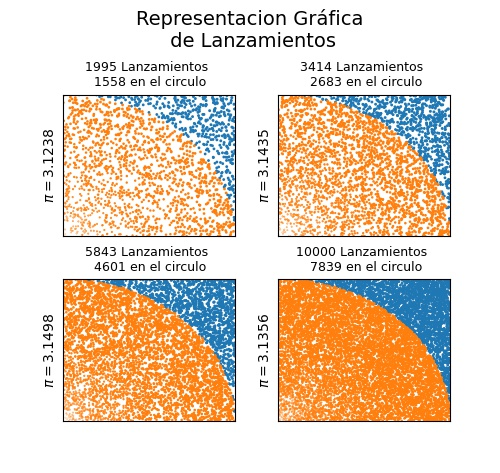
\includegraphics[width=\linewidth]{figures/areas}
  \caption{Representación gráfica de como se definen areas para el cálculo de Pi}
  \label{area}
\end{figure}


Queda bastante ejemplificado que mientras mayor sea el número de puntos, las áreas quedan mejor definidas.
Para obtener esta aproximación se necesitan generar los puntos aleatoriamente con una distribución uniforme, es decir, con igual probabilidad de caer dentro y fuera del área del cuarto de circunferencia.

\subsubsection{Método de Buffon para la estimación de Pi}

En el caso de la estimación de Pi usando la propuesta experimental de Buffon y su extensión de Laplace, tenemos más variables aleatorias a considerar. Puesto que cada aguja, con un centro en (𝑥𝑖,𝑦𝑖), tiene relacionada otra variable aleatoria que corresponde al ángulo de inclinación 𝜃 de la aguja.

Si bien en este caso se recurre a una función trigonométrica para evaluar la inclinación y considerar a las agujas que cruzan la línea, el ordenador usa recursivamente el valor de Pi para calcular la función coseno, siendo este un error “histórico” ya que recurre al valor de pi para calcular al mismo. Por esta razón se usó una corrección geométrica que evita el uso de funciones trigonométricas.
Pasando de requerir generar aleatoriamente un ángulo θ, a generar aleatoriamente desplazamientos δx y δy. En la siguiente figura se muestra una representación gráfica de cómo se realiza la simulación con un número grande de lanzamientos aleatorios con distribución uniforme.


\begin{table*}[t]
  \caption{A double column table.}
  \label{tab:commands}
  \begin{tabular}{ccl}
    \toprule
    A Wide Command Column & A Random Number & Comments\\
    \midrule
    \verb|\tabular| & 100& The content of a table \\
    \verb|\table|  & 300 & For floating tables within a single column\\
    \verb|\table*| & 400 & For wider floating tables that span two columns\\
    \bottomrule
  \end{tabular}
\end{table*}

\subsection{Tables}

Curabitur vitae nulla dapibus, ornare dolor in, efficitur enim. Cras fermentum facilisis elit vitae egestas. Mauris porta, neque non rutrum efficitur, odio odio faucibus tortor, vitae imperdiet metus quam vitae eros. Proin porta dictum accumsan \autoref{tab:commands}.

Duis cursus maximus facilisis. Integer euismod, purus et condimentum suscipit, augue turpis euismod libero, ac porttitor tellus neque eu enim. Nam vulputate est non tellus efficitur pharetra. Aenean molestie tristique venenatis. Nam congue pulvinar vehicula. Duis lacinia mollis purus, ac aliquet arcu dignissim ac \autoref{tab:freq}. 

\begin{table}[hb]% h asks to places the floating element [h]ere.
  \caption{Frequency of Special Characters}
  \label{tab:freq}
  \begin{tabular}{ccl}
    \toprule
    Non-English or Math & Frequency & Comments\\
    \midrule
    \O & 1 in 1000& For Swedish names\\
    $\pi$ & 1 in 5 & Common in math\\
    \$ & 4 in 5 & Used in business\\
    $\Psi^2_1$ & 1 in 40\,000 & Unexplained usage\\
  \bottomrule
\end{tabular}
\end{table}

Nulla sit amet enim tortor. Ut non felis lectus. Aenean quis felis faucibus, efficitur magna vitae. Curabitur ut mauris vel augue tempor suscipit eget eget lacus. Sed pulvinar lobortis dictum. Aliquam dapibus a velit.

\subsection{Listings and Styles}

Aenean malesuada fringilla felis, vel hendrerit enim feugiat et. Proin dictum ante nec tortor bibendum viverra. Curabitur non nibh ut mauris egestas ultrices consequat non odio.

\begin{itemize}
\item Duis lacinia mollis purus, ac aliquet arcu dignissim ac. Vivamus accumsan sollicitudin dui, sed porta sem consequat.
\item Curabitur ut mauris vel augue tempor suscipit eget eget lacus. Sed pulvinar lobortis dictum. Aliquam dapibus a velit.
\item Curabitur vitae nulla dapibus, ornare dolor in, efficitur enim.
\end{itemize}

Ut sagittis, massa nec rhoncus dignissim, urna ipsum vestibulum odio, ac dapibus massa lorem a dui. Nulla sit amet enim tortor. Ut non felis lectus. Aenean quis felis faucibus, efficitur magna vitae. 

\begin{enumerate}
\item Duis lacinia mollis purus, ac aliquet arcu dignissim ac. Vivamus accumsan sollicitudin dui, sed porta sem consequat.
\item Curabitur ut mauris vel augue tempor suscipit eget eget lacus. Sed pulvinar lobortis dictum. Aliquam dapibus a velit.
\item Curabitur vitae nulla dapibus, ornare dolor in, efficitur enim.
\end{enumerate}

Cras fermentum facilisis elit vitae egestas. Mauris porta, neque non rutrum efficitur, odio odio faucibus tortor, vitae imperdiet metus quam vitae eros. Proin porta dictum accumsan. Aliquam dapibus a velit. Curabitur vitae nulla dapibus, ornare dolor in, efficitur enim. Ut maximus mi id arcu ultricies feugiat. Phasellus facilisis purus ac ipsum varius bibendum.

\subsection{Math and Equations}

Curabitur vitae nulla dapibus, ornare dolor in, efficitur enim. Cras fermentum facilisis elit vitae egestas. Nam vulputate est non tellus efficitur pharetra. Vestibulum ligula est, varius in suscipit vel, porttitor id massa. Cras facilisis suscipit orci, ac tincidunt erat.
\begin{equation}
  \lim_{n\rightarrow \infty}x=0
\end{equation}

Sed pulvinar lobortis dictum. Aliquam dapibus a velit porttitor ultrices. Ut maximus mi id arcu ultricies feugiat. Phasellus facilisis purus ac ipsum varius bibendum. Aenean a quam at massa efficitur tincidunt facilisis sit amet felis. 
\begin{displaymath}
  \sum_{i=0}^{\infty} x + 1
\end{displaymath}

Suspendisse molestie ultricies tincidunt. Praesent metus ex, tempus quis gravida nec, consequat id arcu. Donec maximus fermentum nulla quis maximus.
$ \sum_{i=0}^{\infty}x_i=\int_{0}^{\pi+2} f$

Curabitur vitae nulla dapibus, ornare dolor in, efficitur enim. Cras fermentum facilisis elit vitae egestas. Nam vulputate est non tellus efficitur pharetra. Vestibulum ligula est, varius in suscipit vel, porttitor id massa. Cras facilisis suscipit orci, ac tincidunt erat.

\section{Citations}

Some examples of references. A paginated journal article~\cite{Abril07}, an enumerated journal article~\cite{Cohen07}, a reference to an entire issue~\cite{JCohen96}, a monograph (whole book) ~\cite{Kosiur01}, a monograph/whole book in a series (see 2a in spec. document)~\cite{Harel79}, a divisible-book such as an anthology or compilation~\cite{Editor00} followed by the same example, however we only output the series if the volume number is given~\cite{Editor00a} (so Editor00a's series should NOT be present since it has no vol. no.), a chapter in a divisible book~\cite{Spector90}, a chapter in a divisible book in a series~\cite{Douglass98}, a multi-volume work as book~\cite{Knuth97}, an article in a proceedings (of a conference, symposium, workshop for example) (paginated proceedings article)~\cite{Andler79}, a proceedings article with all possible elements~\cite{Smith10}, an example of an enumerated proceedings article~\cite{VanGundy07}, an informally published work~\cite{Harel78}, a doctoral dissertation~\cite{Clarkson85}, a master's thesis~\cite{anisi03}, an finally two online documents or world wide web resources~\cite{Thornburg01, Ablamowicz07}.

\begin{acks}
 This work was supported by the [...] Research Fund of [...] (Number [...]). Additional funding was provided by [...] and [...]. We also thank [...] for contributing [...].
\end{acks}

%\clearpage

\bibliographystyle{ACM-Reference-Format}
\bibliography{sample}

\end{document}
\endinput
